\documentclass[tikz,border=10pt]{standalone}
\usepackage[T1]{fontenc}
\usepackage[utf8]{inputenc}
\usepackage{lmodern}
\renewcommand\familydefault{\sfdefault}
\usetikzlibrary{positioning,fit,backgrounds,arrows.meta,calc}

\definecolor{src}{HTML}{DBEAFE}   \definecolor{srcb}{HTML}{3B82F6}
\definecolor{proc}{HTML}{F1F5F9}  \definecolor{procb}{HTML}{64748B}
\definecolor{llm}{HTML}{FFEDD5}   \definecolor{llmb}{HTML}{EA580C}
\definecolor{resc}{HTML}{DCFCE7}   \definecolor{rescb}{HTML}{16A34A}
\definecolor{net}{HTML}{F3E8FF}   \definecolor{netb}{HTML}{9333EA}
\definecolor{store}{HTML}{FEF9C3} \definecolor{storeb}{HTML}{CA8A04}

\begin{document}
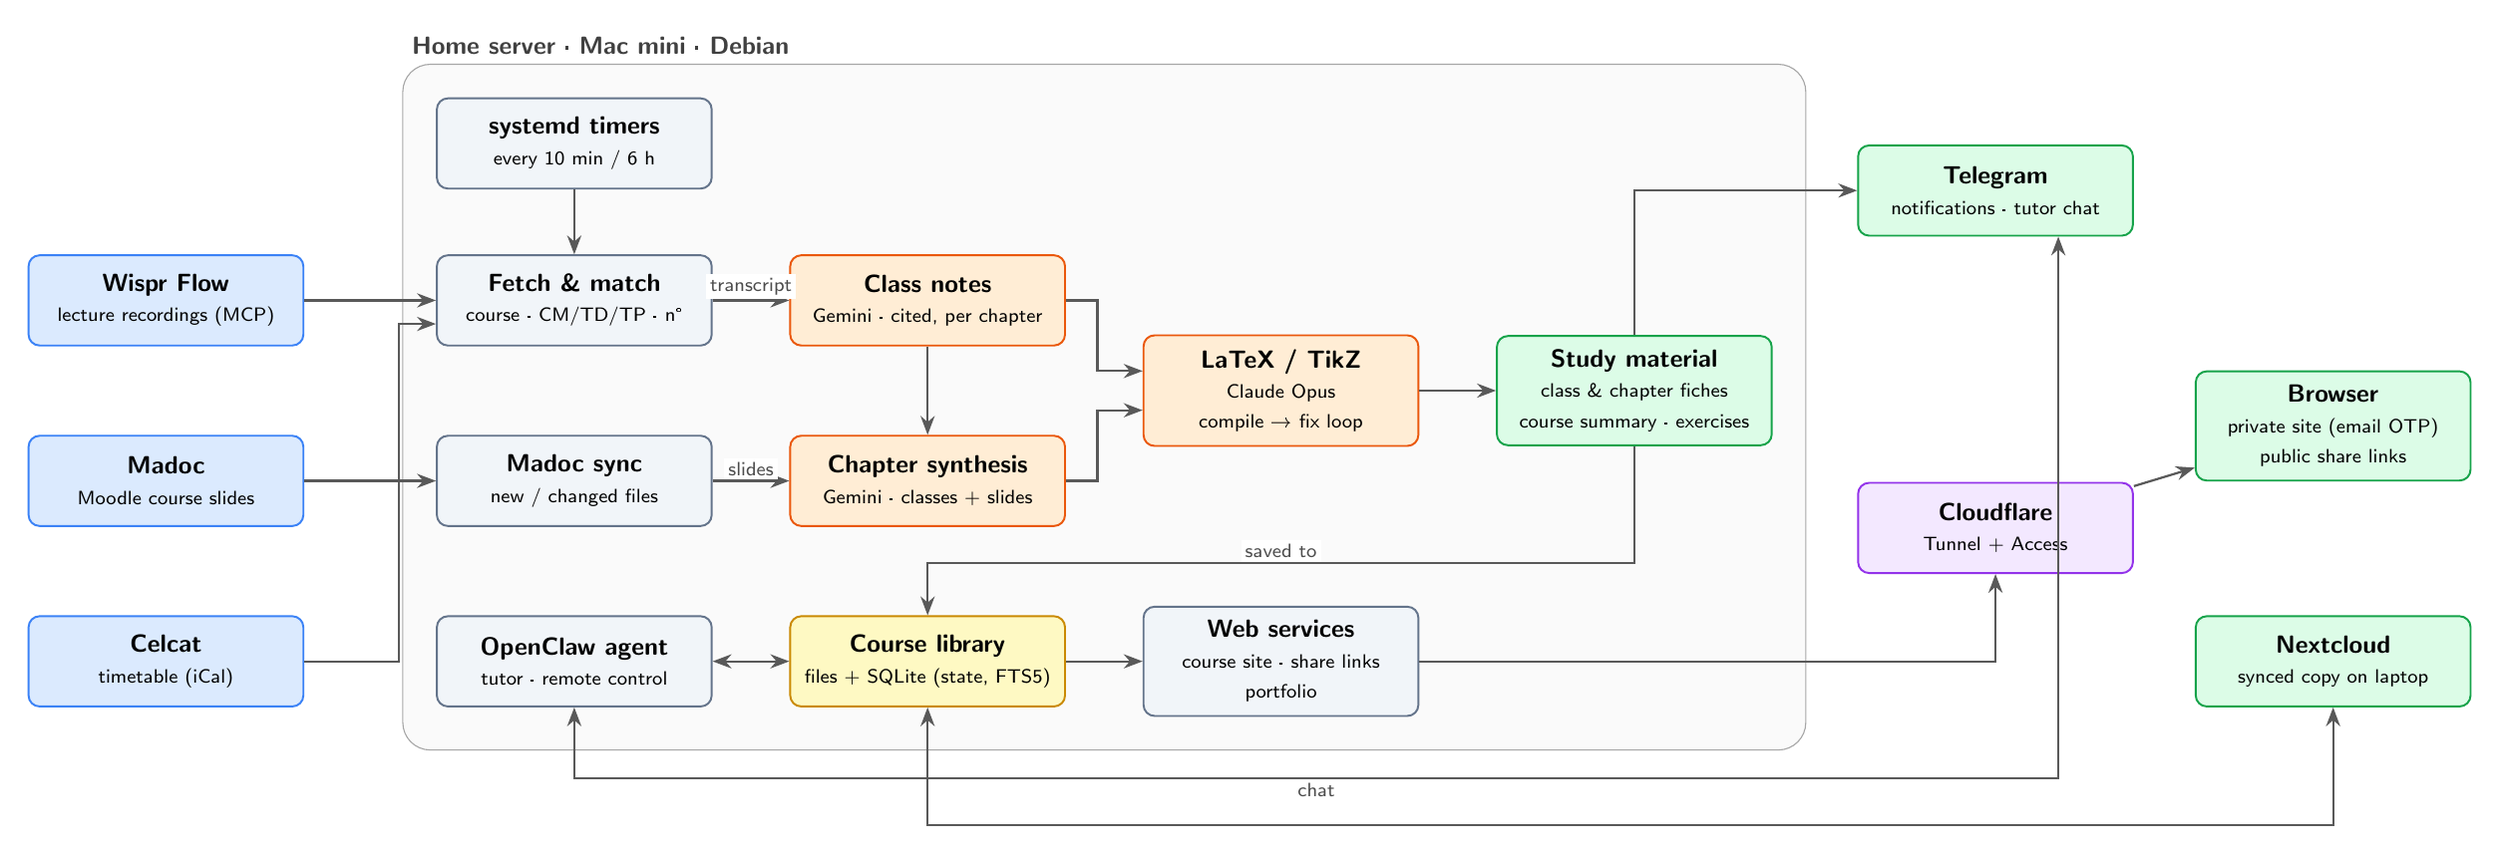
\begin{tikzpicture}[
  font=\small, node distance=6mm and 9mm,
  box/.style={draw, rounded corners=4pt, align=center, minimum width=3.5cm, minimum height=1.15cm, inner sep=5pt, line width=.7pt},
  src/.style={box, fill=src, draw=srcb}, proc/.style={box, fill=proc, draw=procb},
  llm/.style={box, fill=llm, draw=llmb}, res/.style={box, fill=resc, draw=rescb},
  net/.style={box, fill=net, draw=netb}, store/.style={box, fill=store, draw=storeb},
  flow/.style={-{Stealth[length=2.4mm]}, line width=.8pt, black!65},
  both/.style={{Stealth[length=2.4mm]}-{Stealth[length=2.4mm]}, line width=.8pt, black!65},
  lbl/.style={font=\scriptsize, fill=white, inner sep=1.5pt, text=black!70},
  title/.style={font=\bfseries\small, text=black!75},
]

% ---------------- sources
\node[src] (wispr) at (0,4.6) {\textbf{Wispr Flow}\\\scriptsize lecture recordings (MCP)};
\node[src] (madoc) at (0,2.3) {\textbf{Madoc}\\\scriptsize Moodle course slides};
\node[src] (edt)   at (0,0)   {\textbf{Celcat}\\\scriptsize timetable (iCal)};

% ---------------- home server
\node[proc] (fetch)   at (5.2,4.6) {\textbf{Fetch \& match}\\\scriptsize course · CM/TD/TP · n°};
\node[proc] (sync)    at (5.2,2.3) {\textbf{Madoc sync}\\\scriptsize new / changed files};
\node[llm]  (notes)   at (9.7,4.6) {\textbf{Class notes}\\\scriptsize Gemini · cited, per chapter};
\node[llm]  (synth)   at (9.7,2.3) {\textbf{Chapter synthesis}\\\scriptsize Gemini · classes + slides};
\node[llm]  (latex)   at (14.2,3.45) {\textbf{LaTeX / TikZ}\\\scriptsize Claude Opus\\\scriptsize compile → fix loop};
\node[res]  (docs)    at (18.7,3.45) {\textbf{Study material}\\\scriptsize class \& chapter fiches\\\scriptsize course summary · exercises};
\node[store](cours)   at (9.7,0)  {\textbf{Course library}\\\scriptsize files + SQLite (state, FTS5)};
\node[proc] (web)     at (14.2,0) {\textbf{Web services}\\\scriptsize course site · share links\\\scriptsize portfolio};
\node[proc] (agent)   at (5.2,0)  {\textbf{OpenClaw agent}\\\scriptsize tutor · remote control};
\node[proc] (timers)  at (5.2,6.6) {\textbf{systemd timers}\\\scriptsize every 10 min / 6 h};

\begin{scope}[on background layer]
  \node[draw=black!35, fill=black!2, rounded corners=10pt, inner sep=12pt,
        fit=(fetch)(sync)(notes)(synth)(latex)(docs)(cours)(web)(agent)(timers)] (mini) {};
\end{scope}
\node[title, anchor=south west] at (mini.north west) {Home server · Mac mini · Debian};

% ---------------- edge / outputs
\node[net] (cf)   at (23.3,1.7) {\textbf{Cloudflare}\\\scriptsize Tunnel + Access};
\node[res] (tg)   at (23.3,6.0) {\textbf{Telegram}\\\scriptsize notifications · tutor chat};
\node[res] (web2) at (27.6,3.0) {\textbf{Browser}\\\scriptsize private site (email OTP)\\\scriptsize public share links};
\node[res] (nc)   at (27.6,0.0) {\textbf{Nextcloud}\\\scriptsize synced copy on laptop};

% ---------------- flows
\draw[flow] (wispr) -- (fetch);
\draw[flow] (edt.east) -- ++(1.2,0) |- ([yshift=-3mm]fetch.west);
\draw[flow] (madoc) -- (sync);
\draw[flow] (timers) -- (fetch);
\draw[flow] (fetch) -- node[lbl,above]{transcript} (notes);
\draw[flow] (sync) -- node[lbl,above]{slides} (synth);
\draw[flow] (notes) -- (synth);
\draw[flow] (notes.east) -- ++(4mm,0) |- ([yshift=2.5mm]latex.west);
\draw[flow] (synth.east) -- ++(4mm,0) |- ([yshift=-2.5mm]latex.west);
\draw[flow] (latex) -- (docs);
\draw[flow] (docs.south) -- (docs.south |- 0,1.25) -| node[lbl,pos=.25,above]{saved to} (cours.north);
\draw[flow] (cours) -- (web);
\draw[both] (agent) -- (cours);
\draw[flow] (web.east) -| (cf.south);
\draw[flow] (docs.north) |- (tg.west);
\draw[both] (agent.south) -- ++(0,-.9) -| node[lbl,pos=.25,below]{chat} ([xshift=8mm]tg.south) ;
\draw[flow] (cf) -- (web2);
\draw[both] (cours.south) -- ++(0,-1.5) -| (nc.south);

\end{tikzpicture}
\end{document}
